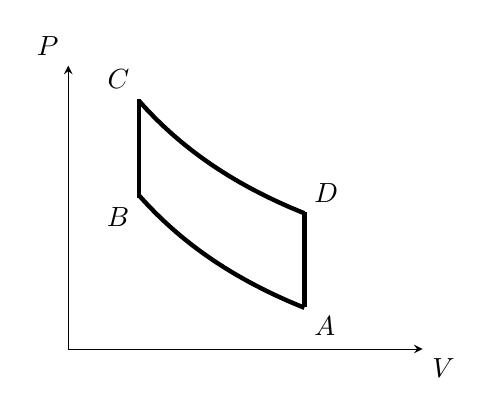
\begin{tikzpicture}[yscale=0.6, xscale=1.5]
\draw [->, >=stealth] (2,-2) --++ (3,0) node[below right]{$V$}; 
\draw [->, >=stealth] (2,-2) --++ (0,6) node[above left]{$P$};
\draw[ultra thick] (2.6,1.2) --++ (0,2.1);
\draw[ultra thick] (4,-1.1) --++ (0,2);
\draw[ultra thick,domain=2.6:4, samples=100] plot ({\x},{20/\x^1.4-2});
\draw[ultra thick,domain=2.6:4, samples=100] plot ({\x},{20/\x^1.4-4});
\draw (2.6,1.2) node[below left]{$B$};
\draw (2.6,3.3) node[above left]{$C$};
\draw (4,-1.1) node[below right]{$A$};
\draw (4,0.9) node[above right]{$D$};
%\draw[domain=2.4:4.5, samples=100] plot ({\x},{20/\x^1.4-2}) node[right]{$isoS$};
%\draw[domain=2:4.5, samples=100] plot ({\x},{20/\x^1.4-4}) node[right]{$isoS$};
%\draw (2.6,-2) -- (2.6,4) node[above]{$isoV$};
%\draw (4,-2) -- (4,2) node[above]{$isoV$};
\end{tikzpicture}